\section{Simulation and Results}

The tests described below were performed in the sequence of the test number. The tests were also performed on the same server without resetting between usages. The goal of the following twenty tests is to be able to verify that our implementation works as expected, and is able to prevent unauthorized tags and clients from completing the protocol all while allowing authorized tags and clients to complete the protocol. These tests were successful in identifying these attacks and avoiding them.

\begin{figure}[H]
    \centering
    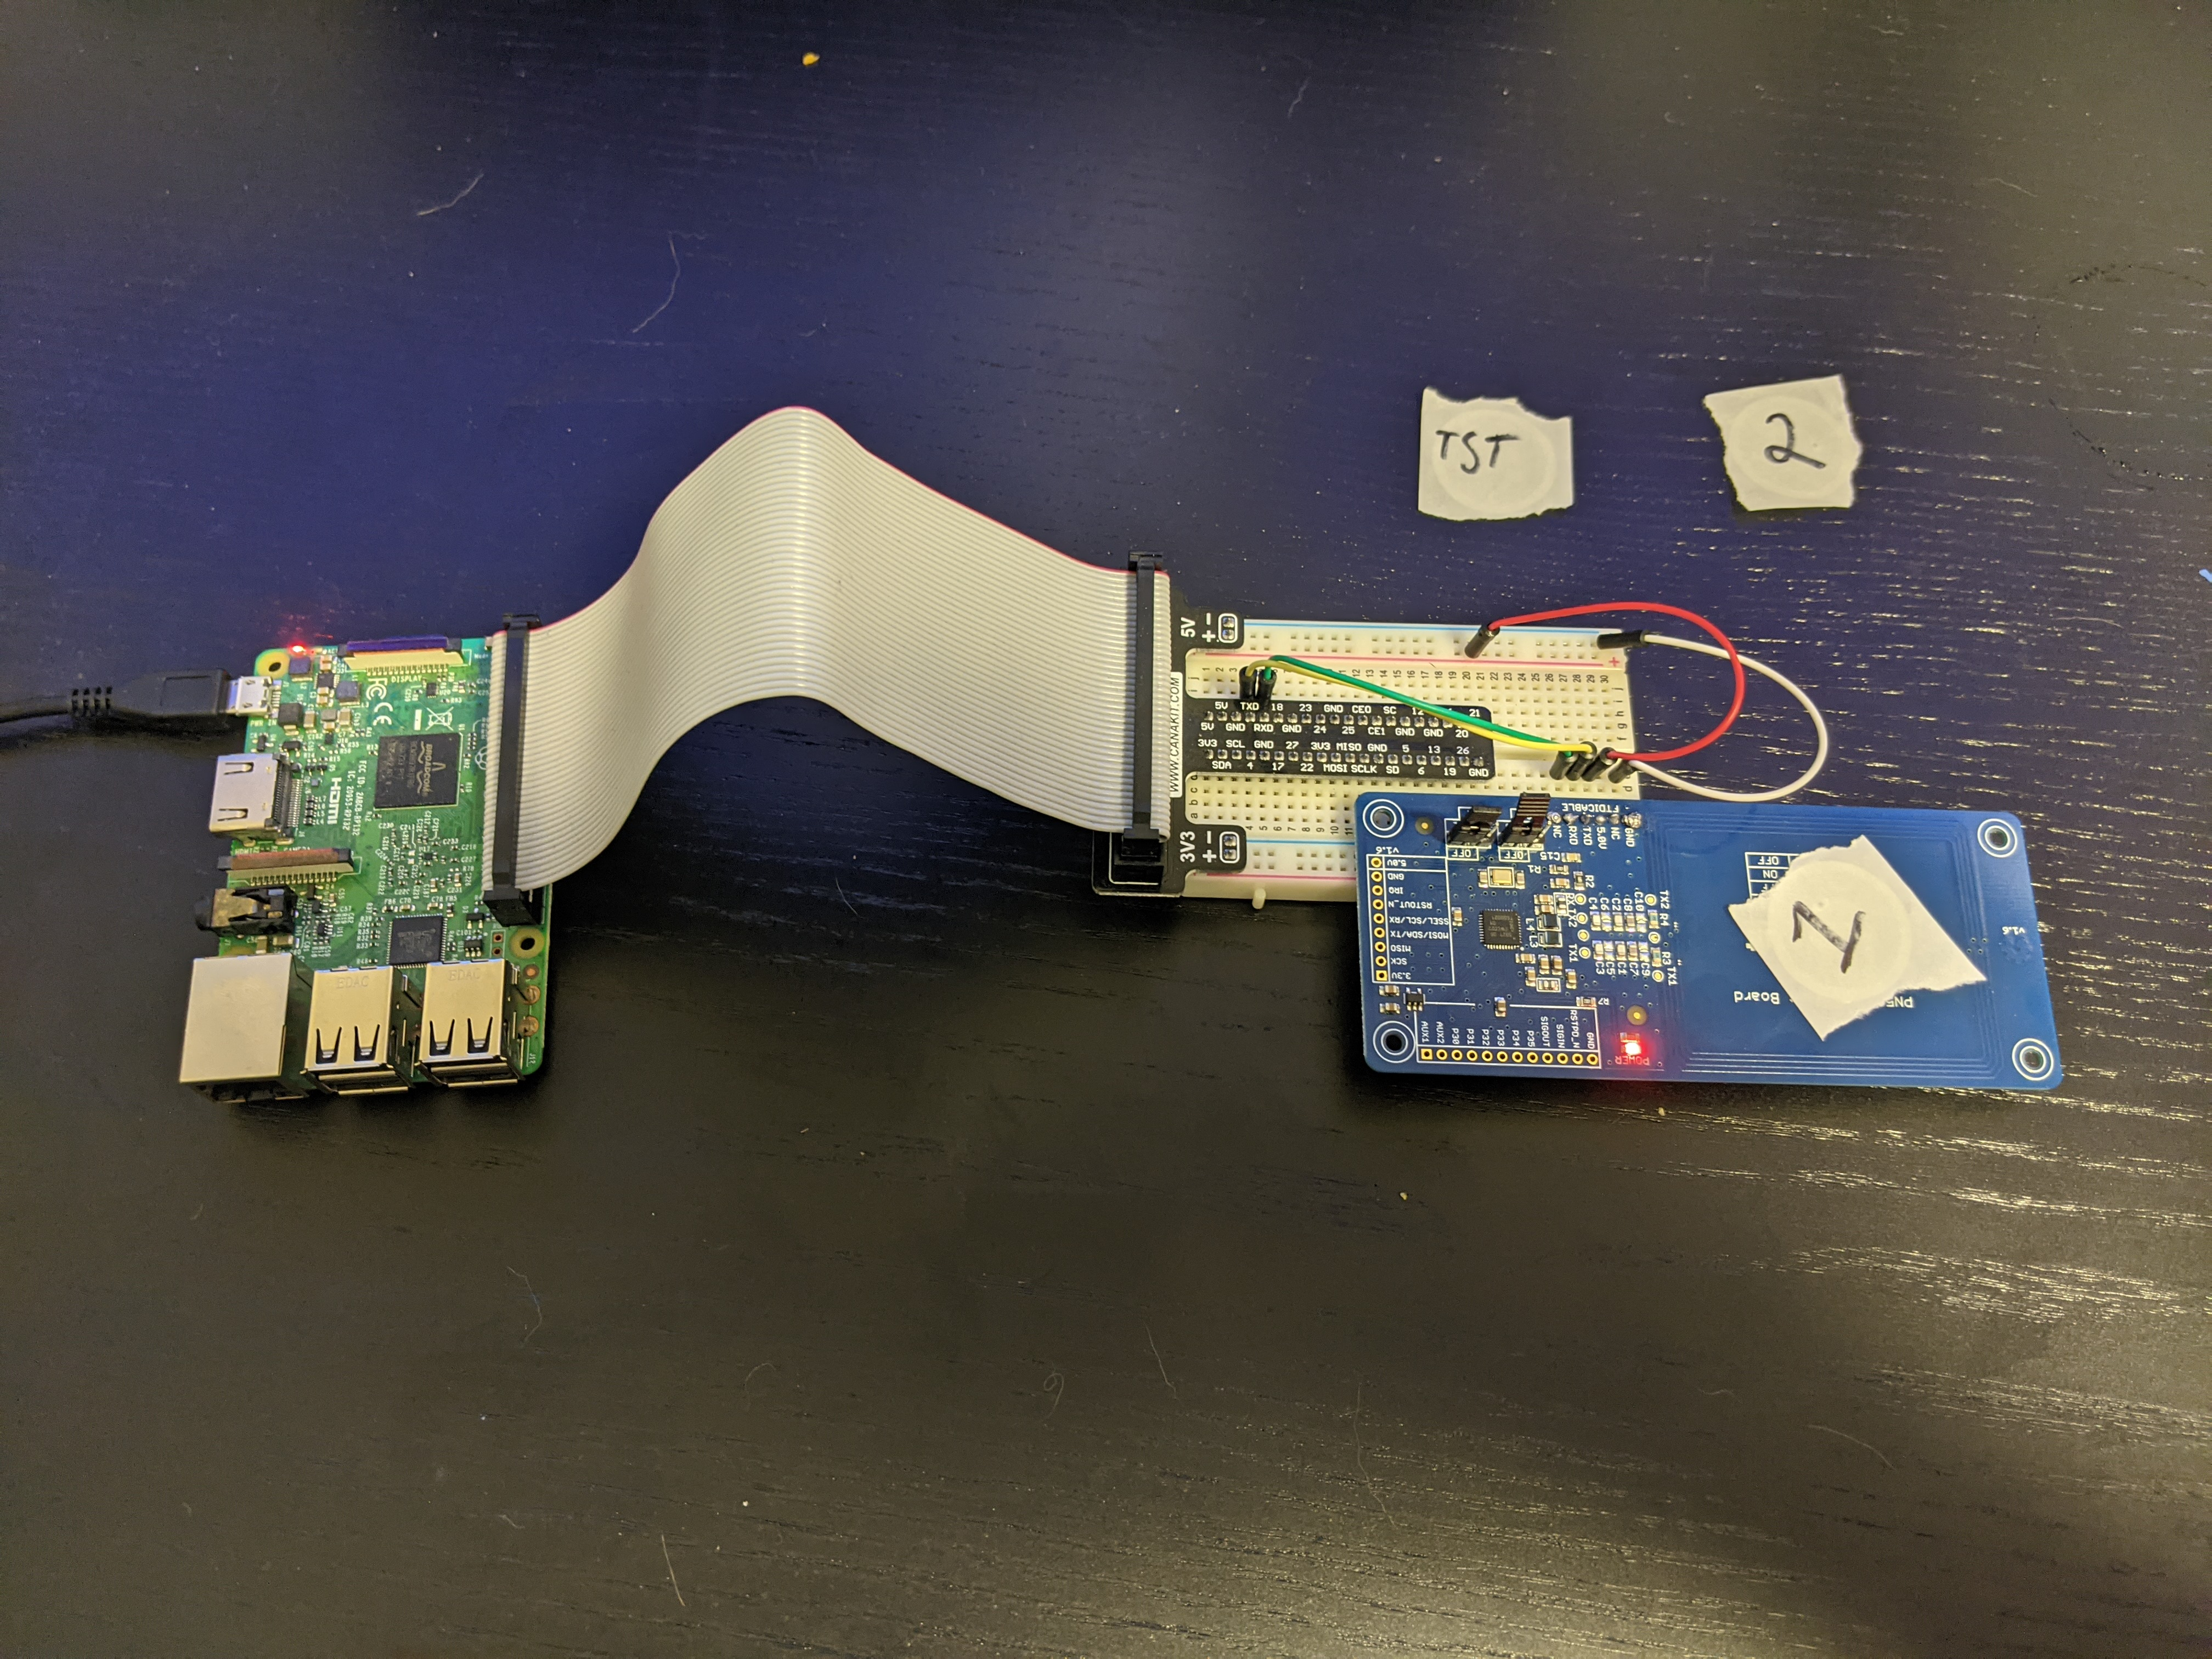
\includegraphics[width=4in]{figures/testing_setup.jpg}
    \caption{Hardware setup for testing tags}
\end{figure}

\subsection{Verification Tests}
\begin{center}
    \begin{tabular}{|c|c|c|c|}
        \hline
        \textbf{Test Number} & \textbf{Test Tag ID} & \textbf{Authentication with Client ID} & \textbf{Results}\\
        \hline
        Test 1 & 1 & 1 & SUCCESS\\
        \hline
        Test 2 & 1 & 2 & SUCCESS\\
        \hline
        Test 3 & 1 & 3 & SUCCESS\\
        \hline
        Test 4 & 2 & 2 & SUCCESS\\
        \hline
        Test 5 & 2 & 3 & SUCCESS\\
        \hline
        Test 6 & 2 & 4 & SUCCESS\\
        \hline
        Test 7 & 3 & 1 & SUCCESS\\
        \hline
        Test 8 & 3 & 2 & SUCCESS\\
        \hline
        Test 9 & 3 & 3 & SUCCESS\\
        \hline
        Test 10 & 4 & 1 & SUCCESS\\
        \hline
    \end{tabular}
\end{center}

The tests performed above were to test the functionality of the client and server as a whole. We used the /auth/client server method to test as it uses both the client and tag information and confirms both at the same time. Success was defined as being able to authenticate the tag and client with the server and correctly updating the random values of both respectfully. Tests one through nine were successful in testing the basic functionality of the developed software by authenticating the client and server at the same time. Test 10 was a confirmation that after test 7 was performed we could re-authenticate the tag and client after additional authentications. 

\subsection{Corrupted Tag Tests}
\begin{center}
    \begin{tabular}{|c|c|c|c|c|c|}
        \hline
        \multicolumn{1}{|p{2cm}|}{\centering \textbf{Test Number} }
        & \multicolumn{1}{|p{2cm}|}{\centering \textbf{Tag ID} }
        & \multicolumn{1}{|p{2cm}|}{\centering \textbf{Original Tag} \\ \textbf{Random Number} \\ }
        & \multicolumn{1}{|p{2cm}|}{\centering \textbf{Corrupted Tag} \\ \textbf{Random Number} \\ }
        & \multicolumn{1}{|p{2.5cm}|}{\centering \textbf{Authentication} \\ \textbf{with Client ID} \\ }
        & \textbf{Results}\\
        \hline
        Test 11 & 1 & 4 & 63 & 4 & SUCCESS\\
        \hline
        Test 12 & 1 & 28 & 63 & 4 & SUCCESS\\
        \hline
        Test 13 & 1 & 63 & 63 & 5 & SUCCESS\\
        \hline
        Test 14 & 1 & 63 & 63 & 5 & SUCCESS\\
        \hline
        Test 15 & 1 & 56 & 63 & 5 & SUCCESS\\
        \hline
    \end{tabular}
\end{center}

The goal of tests eleven through fifteen was to identify if a server could identify a tag that had been tampered with by a malicious actor. To do this test we would first confirm that the tag could be authenticated using the /auth/client server method, then we could corrupt the tag by setting the tag random number to sixty-three. After changing the tag’s data we would then try to authenticate with a valid client, the expected result was failure. Success is defined as being unable to authenticate the client and tag after the tag’s random number had been corrupted/tampered with. For tests 13 and 14, the tags had been previously corrupted in tests 11 and 12 respectively, as such they didn’t have a change in the tag random numbers.

\subsection{Corrupted Client Tests}
\begin{center}
    \begin{tabular}{|c|c|c|c|c|c|}
        \hline
        \multicolumn{1}{|p{2cm}|}{\centering \textbf{Test Number} }
        & \multicolumn{1}{|p{2cm}|}{\centering \textbf{Tag ID} }
        & \multicolumn{1}{|p{2.75cm}|}{\centering \textbf{Authentication} \\ \textbf{with Client ID} \\ }
        & \multicolumn{1}{|p{2cm}|}{\centering \textbf{Original Client} \\ \textbf{Random Number} \\ }
        & \multicolumn{1}{|p{2cm}|}{\centering \textbf{Corrupted Client} \\ \textbf{Random Number} \\ }
        & \textbf{Results}\\
        \hline
        Test 16 & 7 & 6 & 33 & 255 & SUCCESS\\
        \hline
        Test 17 & 8 & 6 & 33 & 255 & SUCCESS\\
        \hline
        Test 18 & 4 & 7 & 4 & 255 & SUCCESS\\
        \hline
        Test 19 & 7 & 7 & 4 & 255 & SUCCESS\\
        \hline
        Test 20 & 8 & 7 & 4 & 255 & SUCCESS\\
        \hline
    \end{tabular}
\end{center}

Finally, our last test set, tests sixteen to twenty is to confirm that a corrupted client could not be authenticated on the server even with a valid tag. These tests used the /auth/client method on the server to attempt to authenticate both the client and tag. The testing method was to first confirm that the client could authenticate with a valid tag, then we would corrupt the client’s data by changing the client random number to two-hundred-fifty-five. Then we would try to authenticate the client with a valid tag, the expected result should be that the authentication fails.